\documentclass[aspectratio=169]{beamer} % Ho mantenuto aspectratio=169 per il formato panoramico

% --- PACCHETTI BASE ---
\usepackage[T1]{fontenc}
\usepackage[utf8]{inputenc}
\usepackage{graphicx}
\usepackage[english]{babel} % Impostato su english poiché le tue slide sono in inglese
\usepackage{booktabs}
\usepackage{amsmath}
\usepackage{xcolor}

% --- IMPOSTAZIONI TEMA E COLORI (Dal tuo template) ---
\usetheme{Ilmenau}
\usecolortheme{beaver}

% Definizione del colore rosso personalizzato
\definecolor{Darkcandyapplered}{rgb}{0.64, 0.0, 0.0}

% Rimozione dei simboli di navigazione in basso a destra
\setbeamertemplate{navigation symbols}{}

% Personalizzazione dei colori per i blocchi e i titoli delle slide
\setbeamercolor{block title}{bg=Darkcandyapplered, fg=white}
\setbeamercolor{frame title}{fg=Darkcandyapplered}

% Personalizzazione del piè di pagina (footline)
\setbeamertemplate{footline}{\leavevmode%
	\begin{beamercolorbox}[wd=.50\paperwidth,left,ht=2.5ex,dp=1.5ex,rightskip=4pt
		plus 1pt, leftskip=4pt]{subsection in head/foot}
		 \insertshortinstitute
	\end{beamercolorbox}%
	\begin{beamercolorbox}[wd=.50\paperwidth,,ht=2.5ex,dp=1.5ex,leftskip=4pt plus 1pt,rightskip=4pt plus 1pt]{section in head/foot}
		\usebeamercolor[fg]{section in foot/head}\insertshortdate\hfill\insertframenumber/\inserttotalframenumber
	\end{beamercolorbox}%
}	

% --- INFORMAZIONI DELLA TESI ---
\title[Multi-Objective PrPA]{Balancing KPIs through Multi-Objective\\Prescriptive Process Analytics}
\subtitle{Master's Thesis Presentation}
\author{Daniele Gelmini}
\institute[UniPD]{Dipartimento di Matematica “Tullio Levi-Civita”\\Università degli Studi di Padova}
\date{August 2026}

\begin{document}

\frame{\titlepage}

\begin{frame}{Background \& Motivation}
    \begin{itemize}
        \item \textbf{Prescriptive Process Analytics (PrPA):} Aims to recommend the next optimal activity and resource to improve Key Performance Indicators (KPIs).
        \item \textbf{Baseline Limitation:} The previous approach aggregates KPIs into a single utility function using an \textit{a priori} $\lambda$ trade-off weight.
        \item \textbf{Drawback:} Training a single predictive model restricts flexibility. Adjusting the strategic trade-off requires completely retraining the model.
    \end{itemize}
\end{frame}

\begin{frame}{Proposed Framework Enhancements}
    \begin{block}{From \textit{A Priori} to \textit{A Posteriori}}
        Instead of selecting $\lambda$ beforehand, the new approach generates multiple optimal solutions, allowing decision-makers to select the desired trade-off \textit{a posteriori} without retraining.
    \end{block}
    \vspace{0.3cm}
    \textbf{Key Modifications:}
    \begin{itemize}
        \item \textbf{Independent Models:} Train a distinct model for each individual KPI.
        \item \textbf{Pareto Front Generation:} Evaluate and store all optimal non-dominated solutions during the recommendation phase.
        \item \textbf{Algorithm Shift:} Replace the previous genetic algorithm with NSGA-II for robust multi-objective optimization.
    \end{itemize}
\end{frame}

\begin{frame}{Model Architectures Comparison}
    \begin{columns}
        \begin{column}{0.5\textwidth}
            \centering
            \textbf{Original Architecture} \\
            \vspace{0.2cm}
            \includegraphics[width=\linewidth]{diagramma_old.png} \\
            \vspace{0.1cm}
            \footnotesize{(Single utility model, \textit{a priori} $\lambda$)}
        \end{column}
        \begin{column}{0.5\textwidth}
            \centering
            \textbf{Proposed Architecture} \\
            \vspace{0.2cm}
            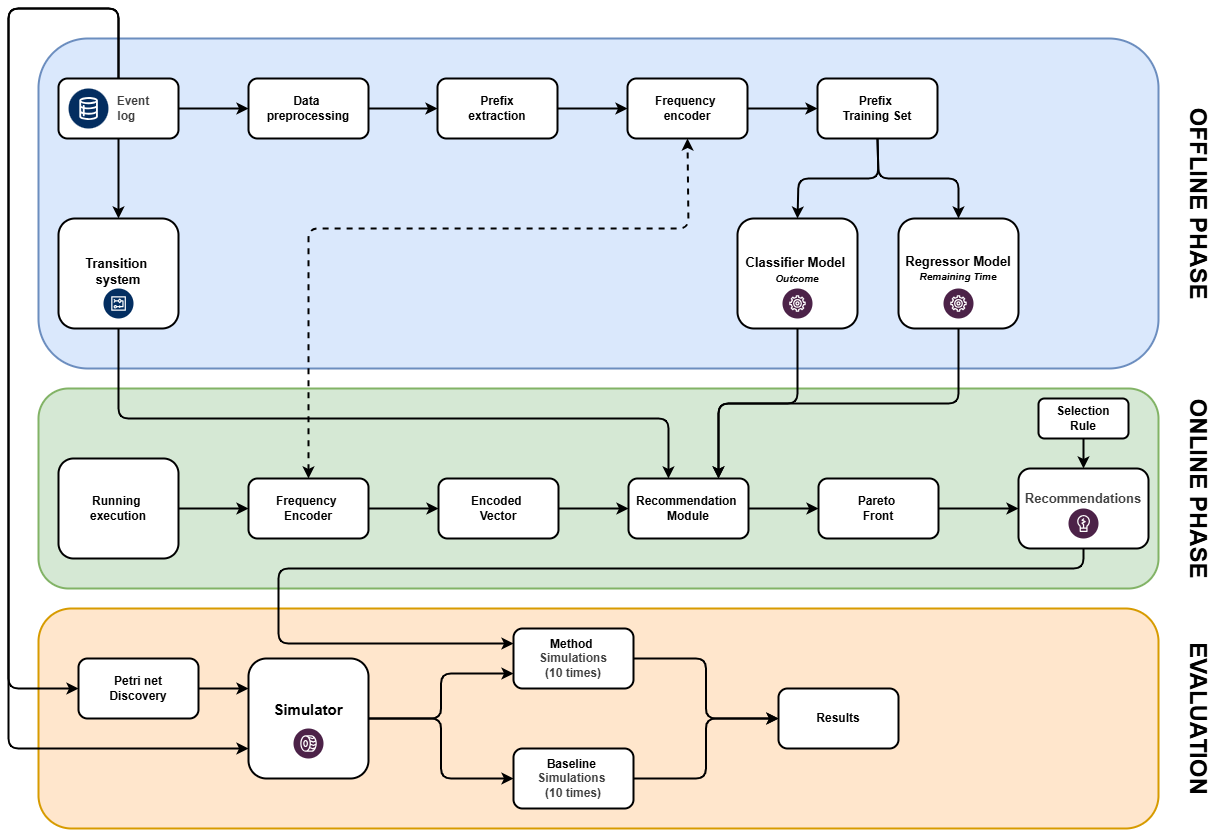
\includegraphics[width=\linewidth]{diagramma.drawio.png} \\
            \vspace{0.1cm}
            \footnotesize{(Multi-model, Pareto Front generation)}
        \end{column}
    \end{columns}
\end{frame}

\section{Offline Phase}

\begin{frame}{Predictive Modeling Strategy}
    \begin{itemize}
        \item The framework leverages independent Machine Learning models tailored to the specific nature of each KPI.
        \item \textbf{Implementation Example:}
        \begin{itemize}
            \item \textbf{CatBoost Regressor:} Used to predict continuous KPIs (e.g., Remaining Execution Time).
            \item \textbf{CatBoost Classifier:} Used to predict discrete or binary KPIs (e.g., Case Outcome probability via \texttt{predict\_proba}).
        \end{itemize}
        \item This decoupling provides higher accuracy and prevents conflicting objectives from diluting a single model's predictive performance.
        \item Both models are trained once, offline, on the encoded prefix training set, and reused for every case and every candidate (activity, resource) pair during the online recommendation phase.
    \end{itemize}
\end{frame}

\section{Online Phase}

\begin{frame}{Recommendation Generation \& NSGA-II}
    \begin{itemize}
        \item While the exhaustive search method remains unchanged as a baseline, the heuristic exploration now employs \textbf{NSGA-II} (Non-dominated Sorting Genetic Algorithm II).
        \item \textbf{Why NSGA-II?} It is explicitly designed for multi-objective optimization, searching for the whole Pareto front in a single run instead of collapsing objectives into one scalar score.
        \item \textbf{Core Mechanisms:}
        \begin{itemize}
            \item \textit{Non-dominated Sorting:} Solutions are ranked into fronts according to Pareto dominance.
            \item \textit{Crowding Distance:} Maintains population diversity by favoring solutions in less crowded regions of the front.
        \end{itemize}
        \item \textbf{No Prior Assumptions:} NSGA-II requires \emph{no} assumption on the objective functions -- no convexity, continuity, differentiability, or \textit{a priori} weighting between outcome and time is needed, unlike scalarization-based approaches.
    \end{itemize}
\end{frame}

\begin{frame}{Exploring the Pareto Front \& Time Normalization}
    \begin{itemize}
        \item \textbf{Time Transformation Pipeline:} To harmonize scales and enable multi-objective optimization, raw remaining time undergoes:
        \begin{enumerate}
            \item \textbf{Z-normalization:} Standardizes skewed temporal distributions.
            \item \textbf{Sigmoid Transformation:} Smooths extreme outliers.
            \item \textbf{Min-Max Scaling:} Maps values into the $[0, 1]$ interval.
        \end{enumerate}
        \item \textbf{Inversion ($1 - \text{Time}$):} Converts time minimization into maximization, placing the ideal theoretical point at $(1,1)$ for intuitive visual trade-off analysis.
    \end{itemize}
\end{frame}

\begin{frame}{Experimental Results: Pareto Fronts (BAC)}
    \centering
    
    \begin{minipage}{0.48\textwidth}
        \centering
        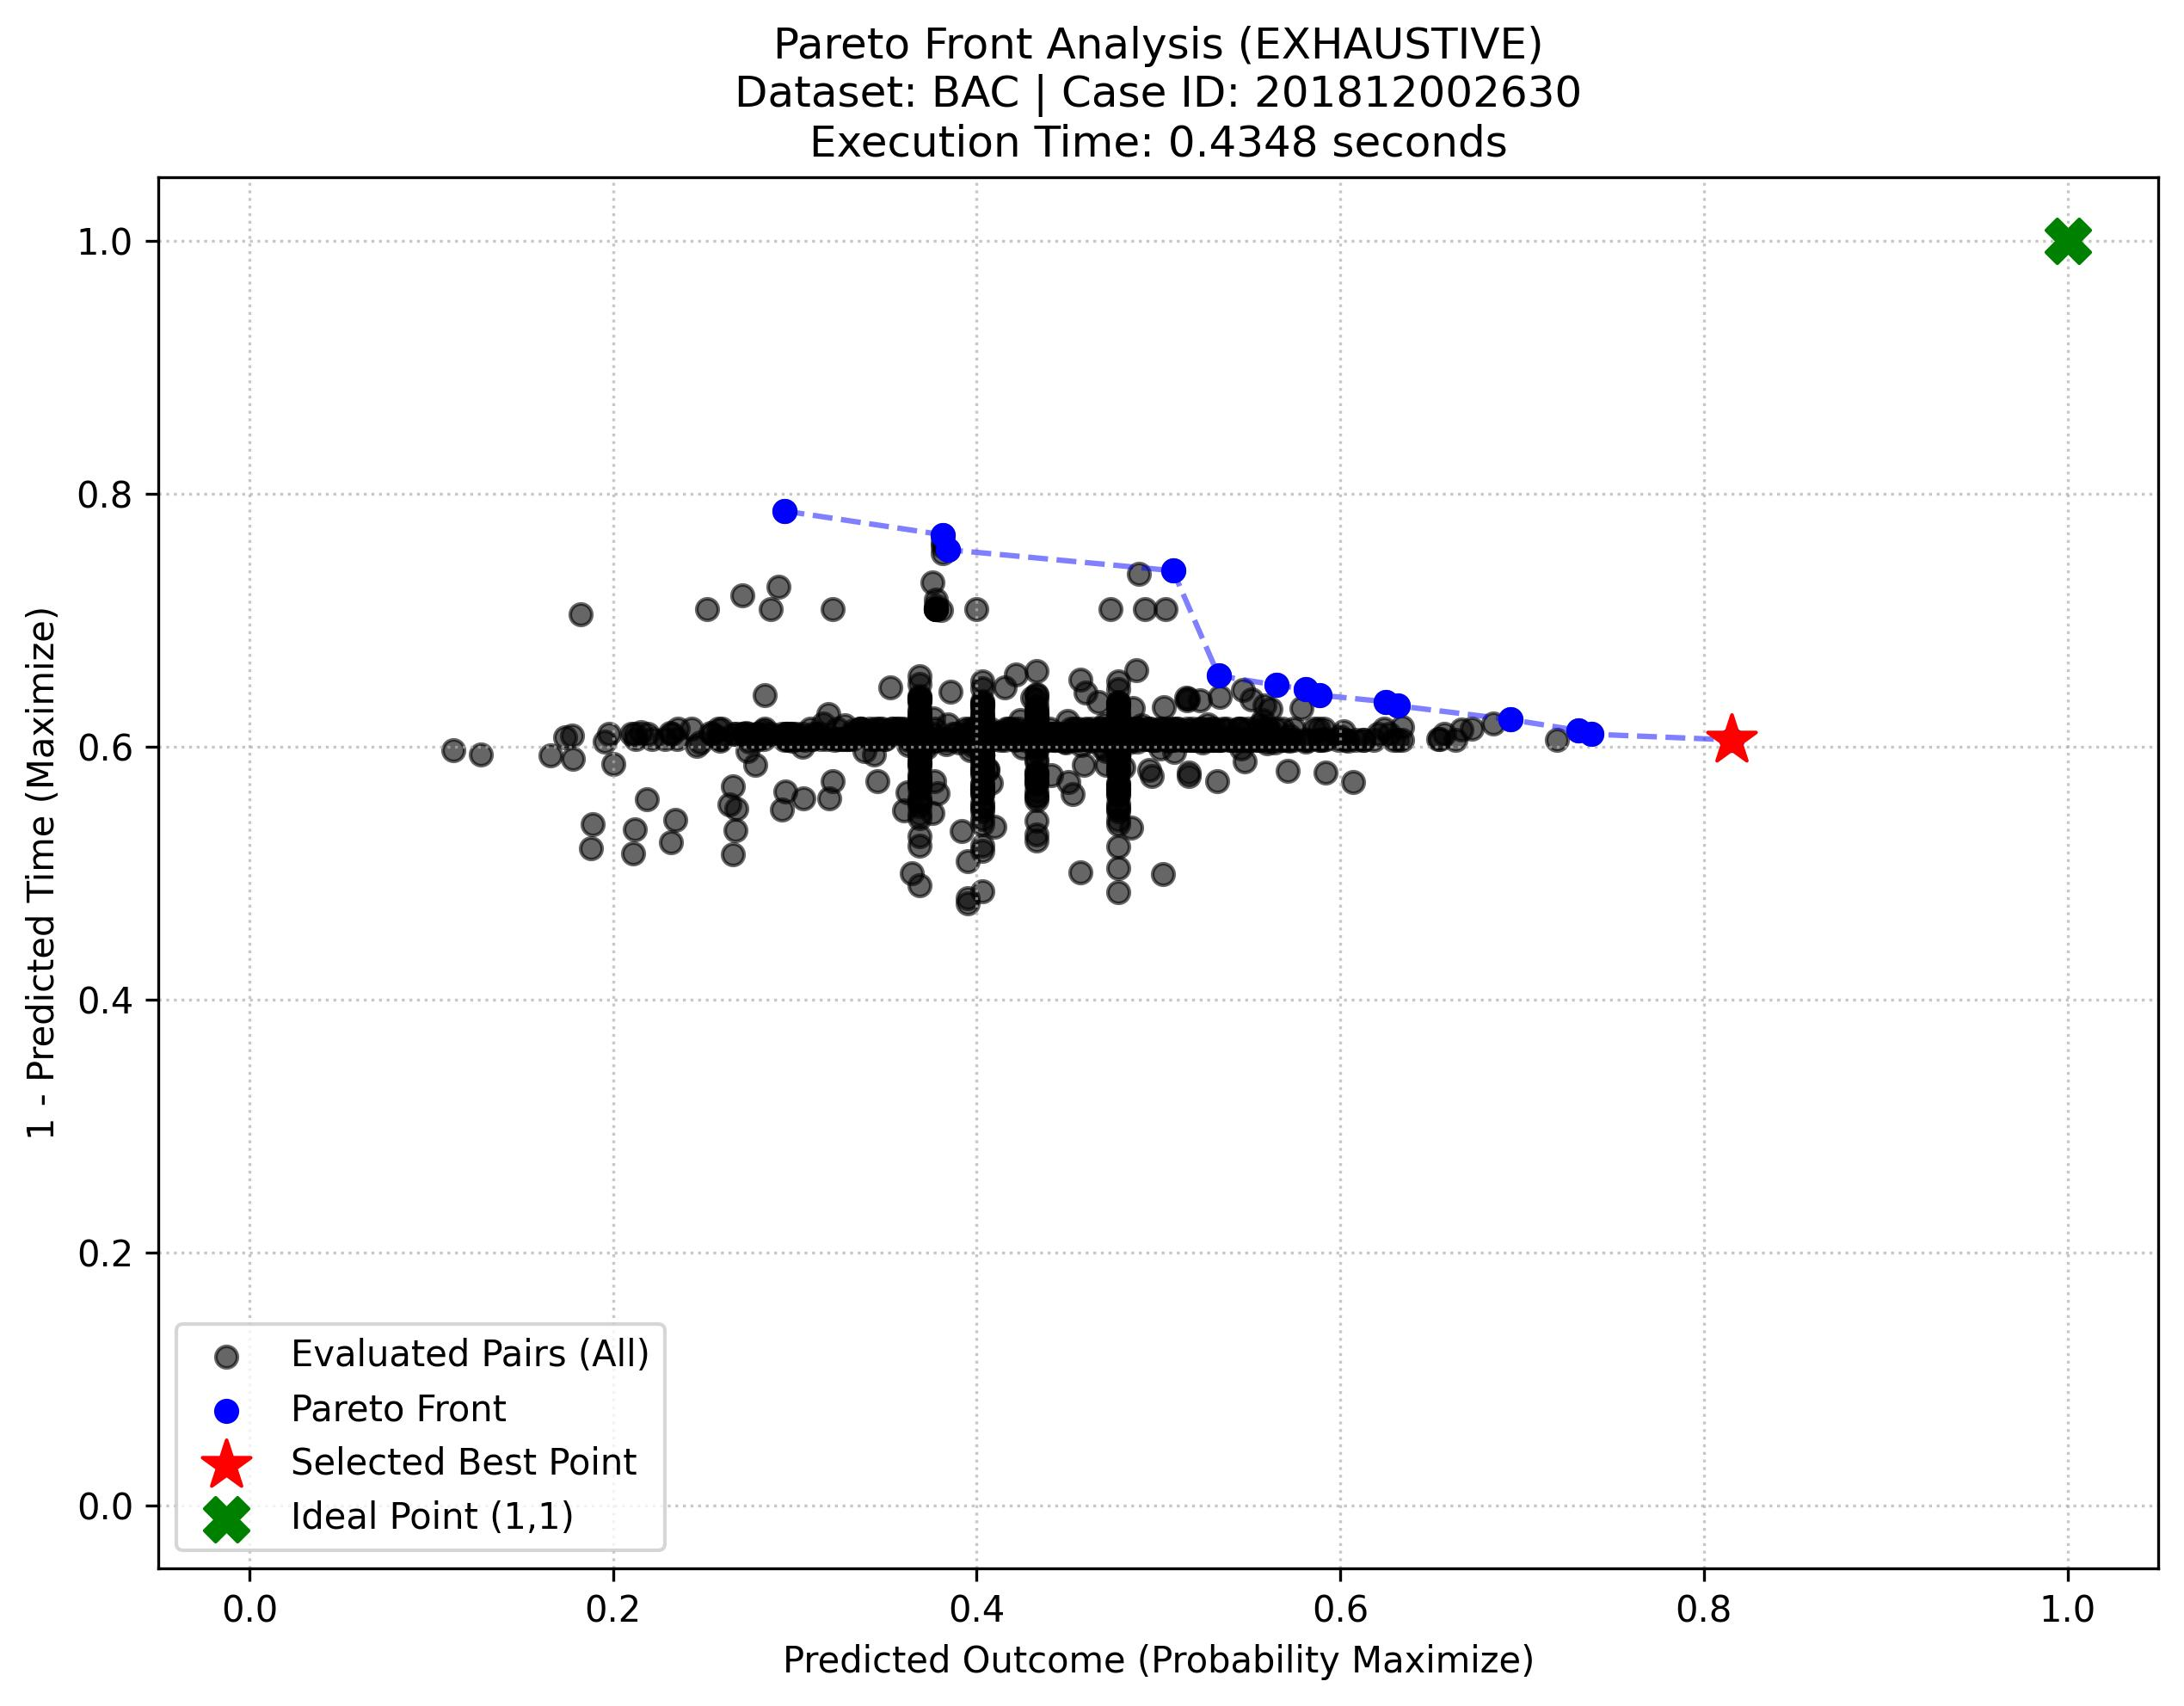
\includegraphics[width=\linewidth]{pareto_front_images/pareto_BAC_exhaustive_201812002630.jpg}
    \end{minipage}
    \begin{minipage}{0.48\textwidth}
        \centering
        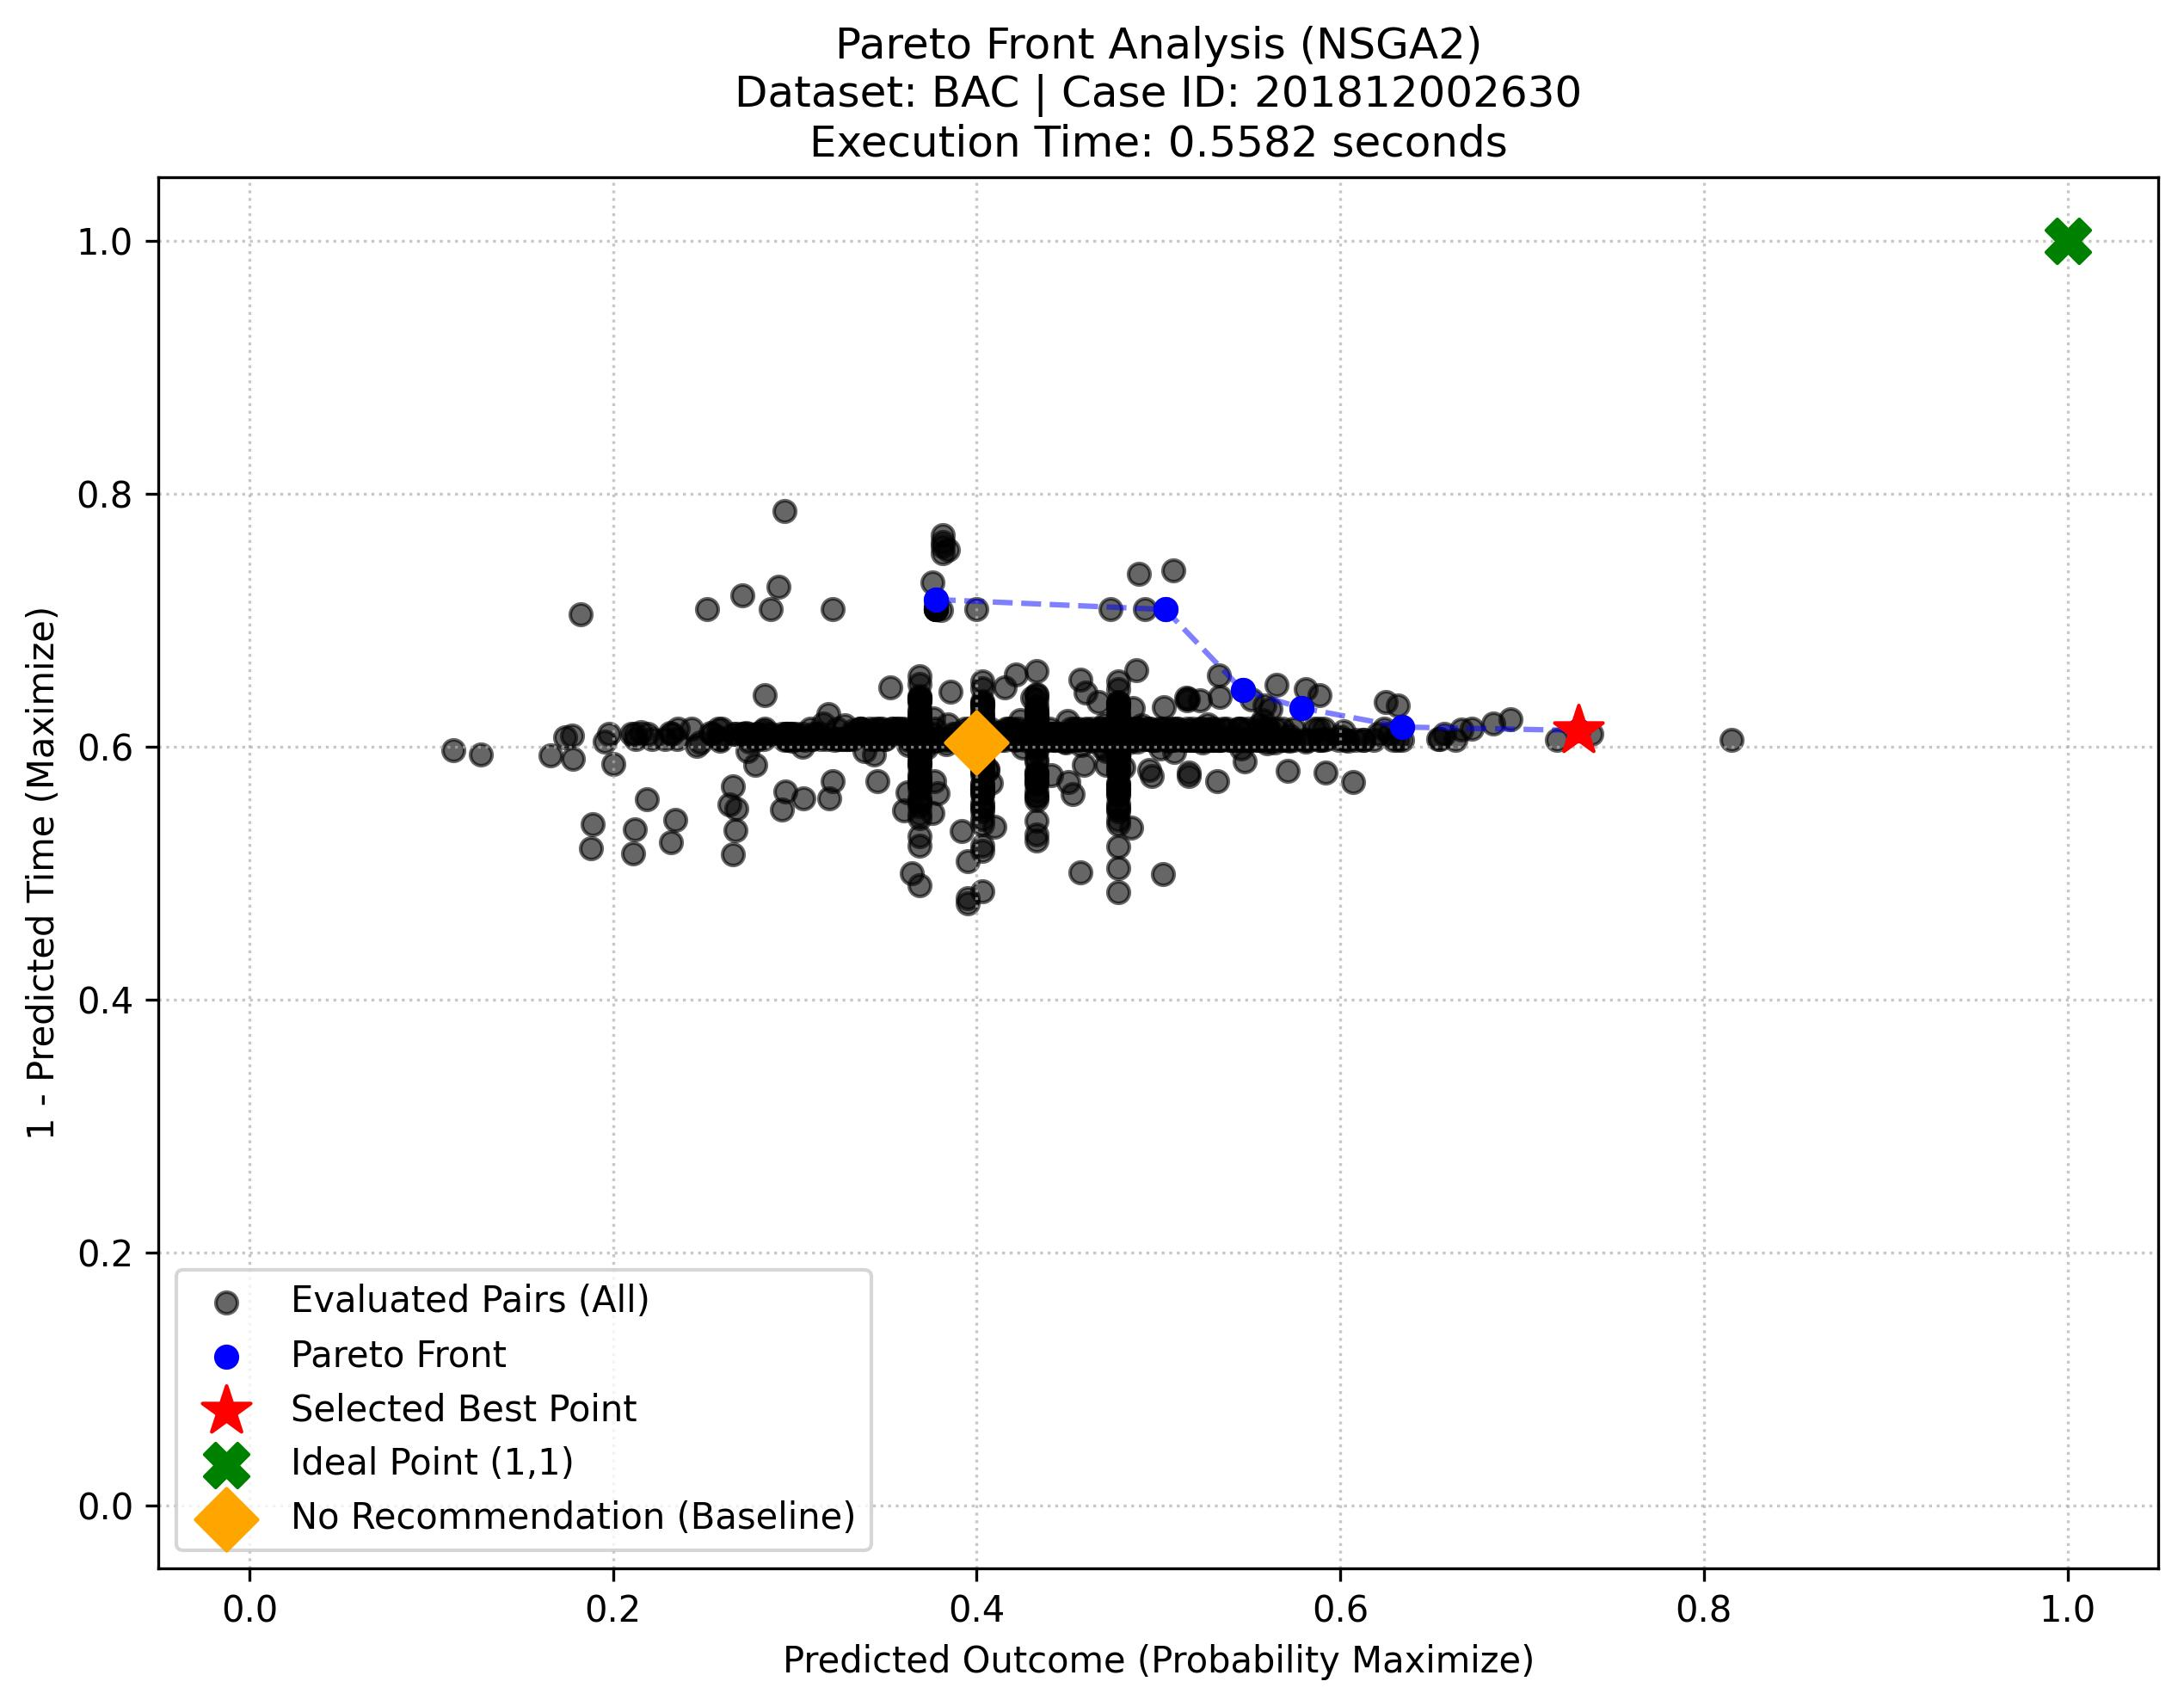
\includegraphics[width=\linewidth]{pareto_front_images/pareto_BAC_nsga2_201812002630.jpg}
    \end{minipage}
    
\end{frame}

\begin{frame}{Experimental Results: Pareto Fronts (BPI12)}
    \centering

    \begin{minipage}{0.48\textwidth}
        \centering
        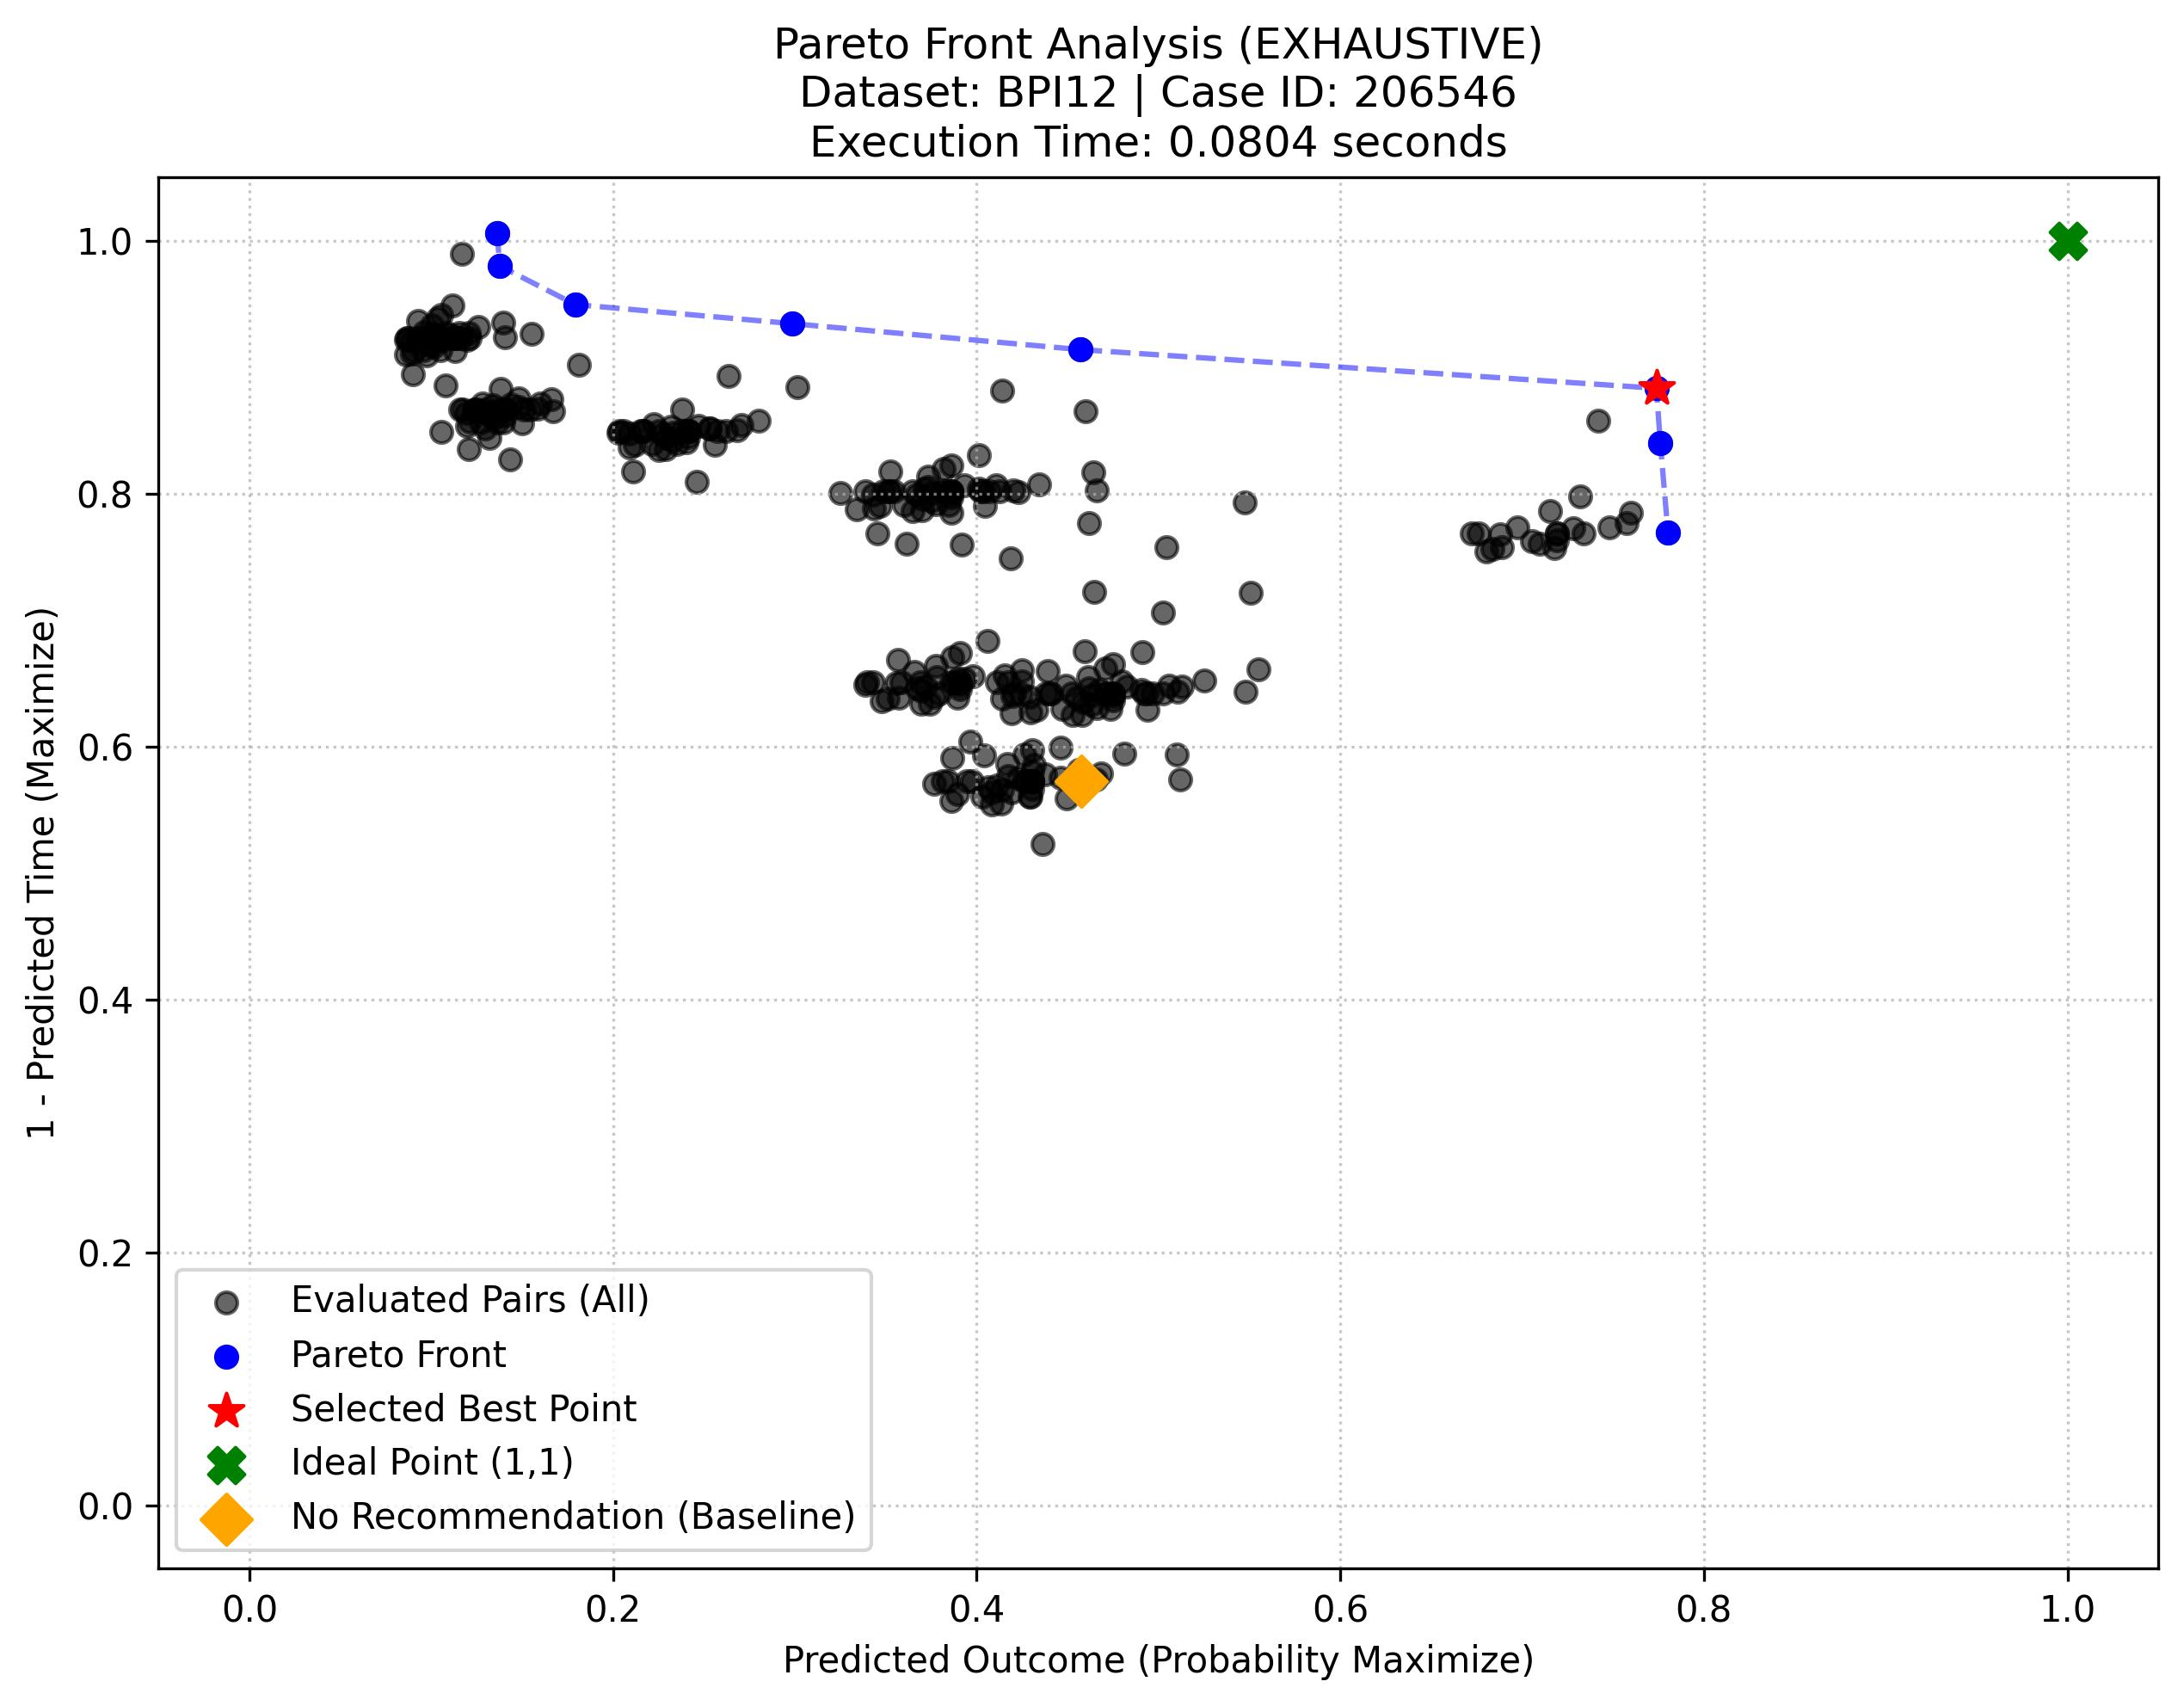
\includegraphics[width=1.03\linewidth]{pareto_front_images/pareto_BPI12_exhaustive_206546.jpg}
    \end{minipage}
    \begin{minipage}{0.48\textwidth}
        \centering
        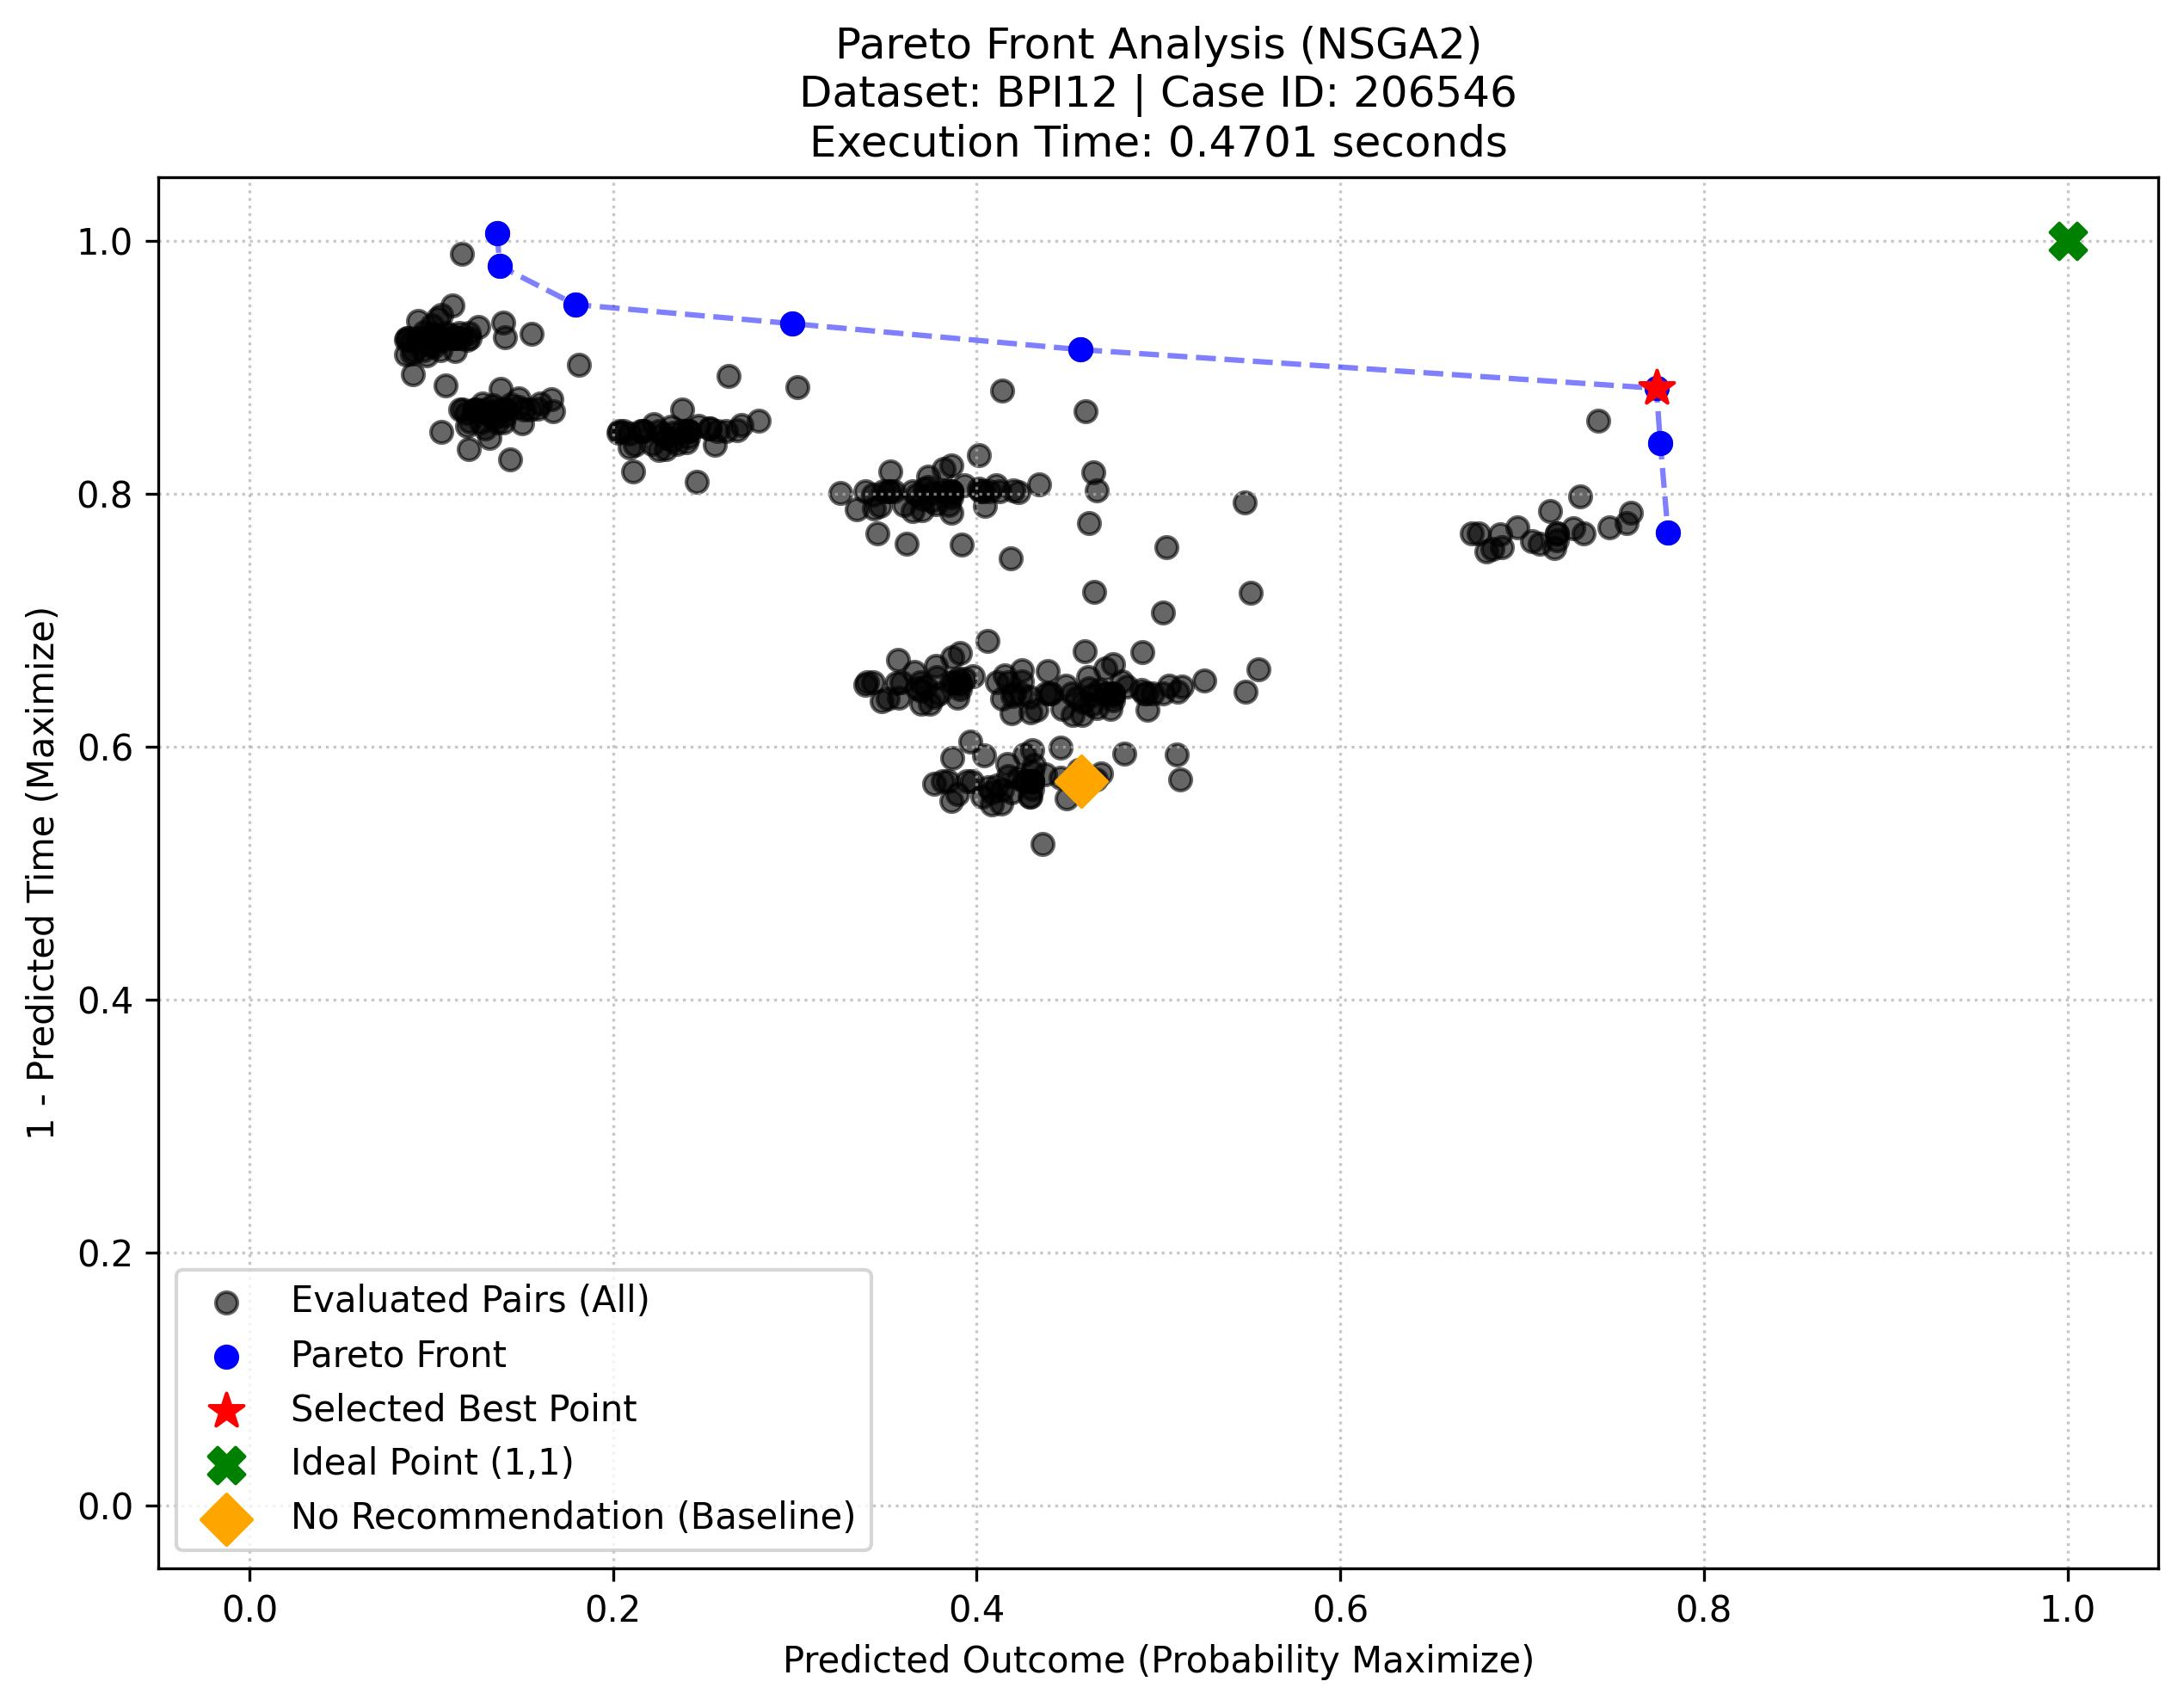
\includegraphics[width=1.03\linewidth]{pareto_front_images/pareto_BPI12_nsga2_206546.jpg}
    \end{minipage}
    
\end{frame}

\begin{frame}{Experimental Results: Pareto Fronts (bpi17-before)}
    \centering
    
    \begin{minipage}{0.48\textwidth}
        \centering
        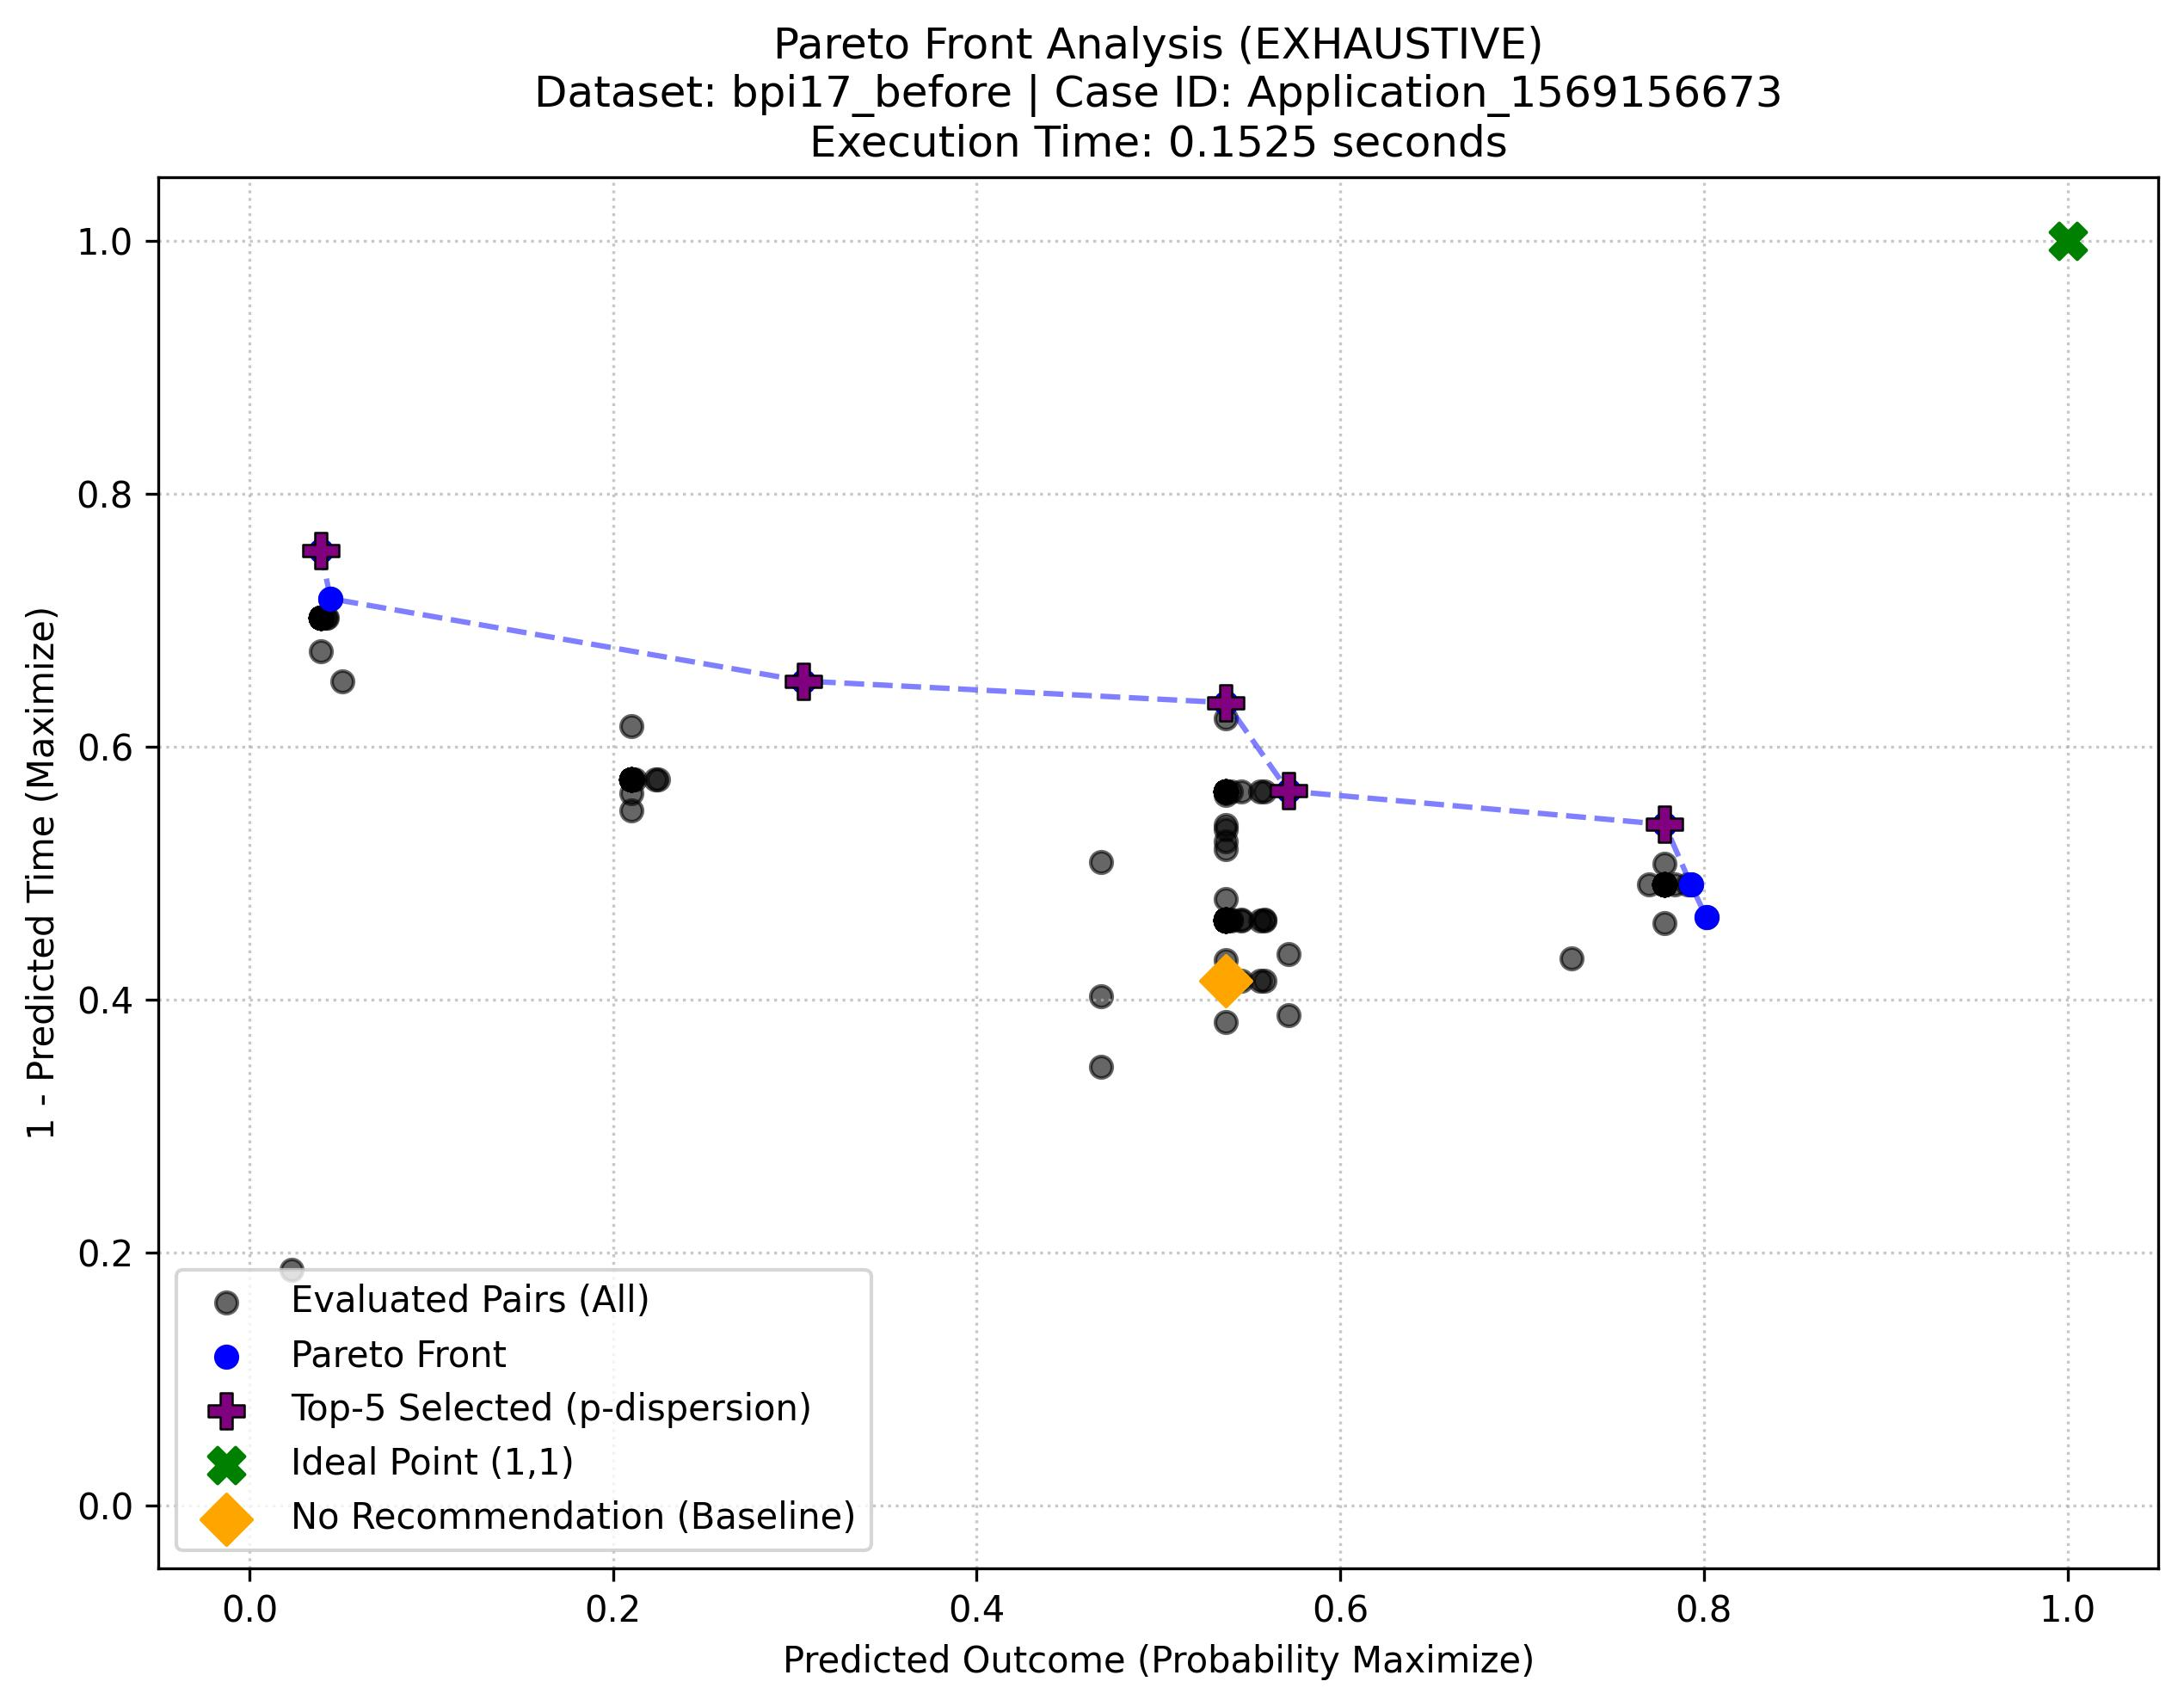
\includegraphics[width=1.03\linewidth]{pareto_front_images/pareto_bpi17_before_exhaustive_Application_1569156673.jpg}
    \end{minipage}
    \begin{minipage}{0.48\textwidth}
        \centering
        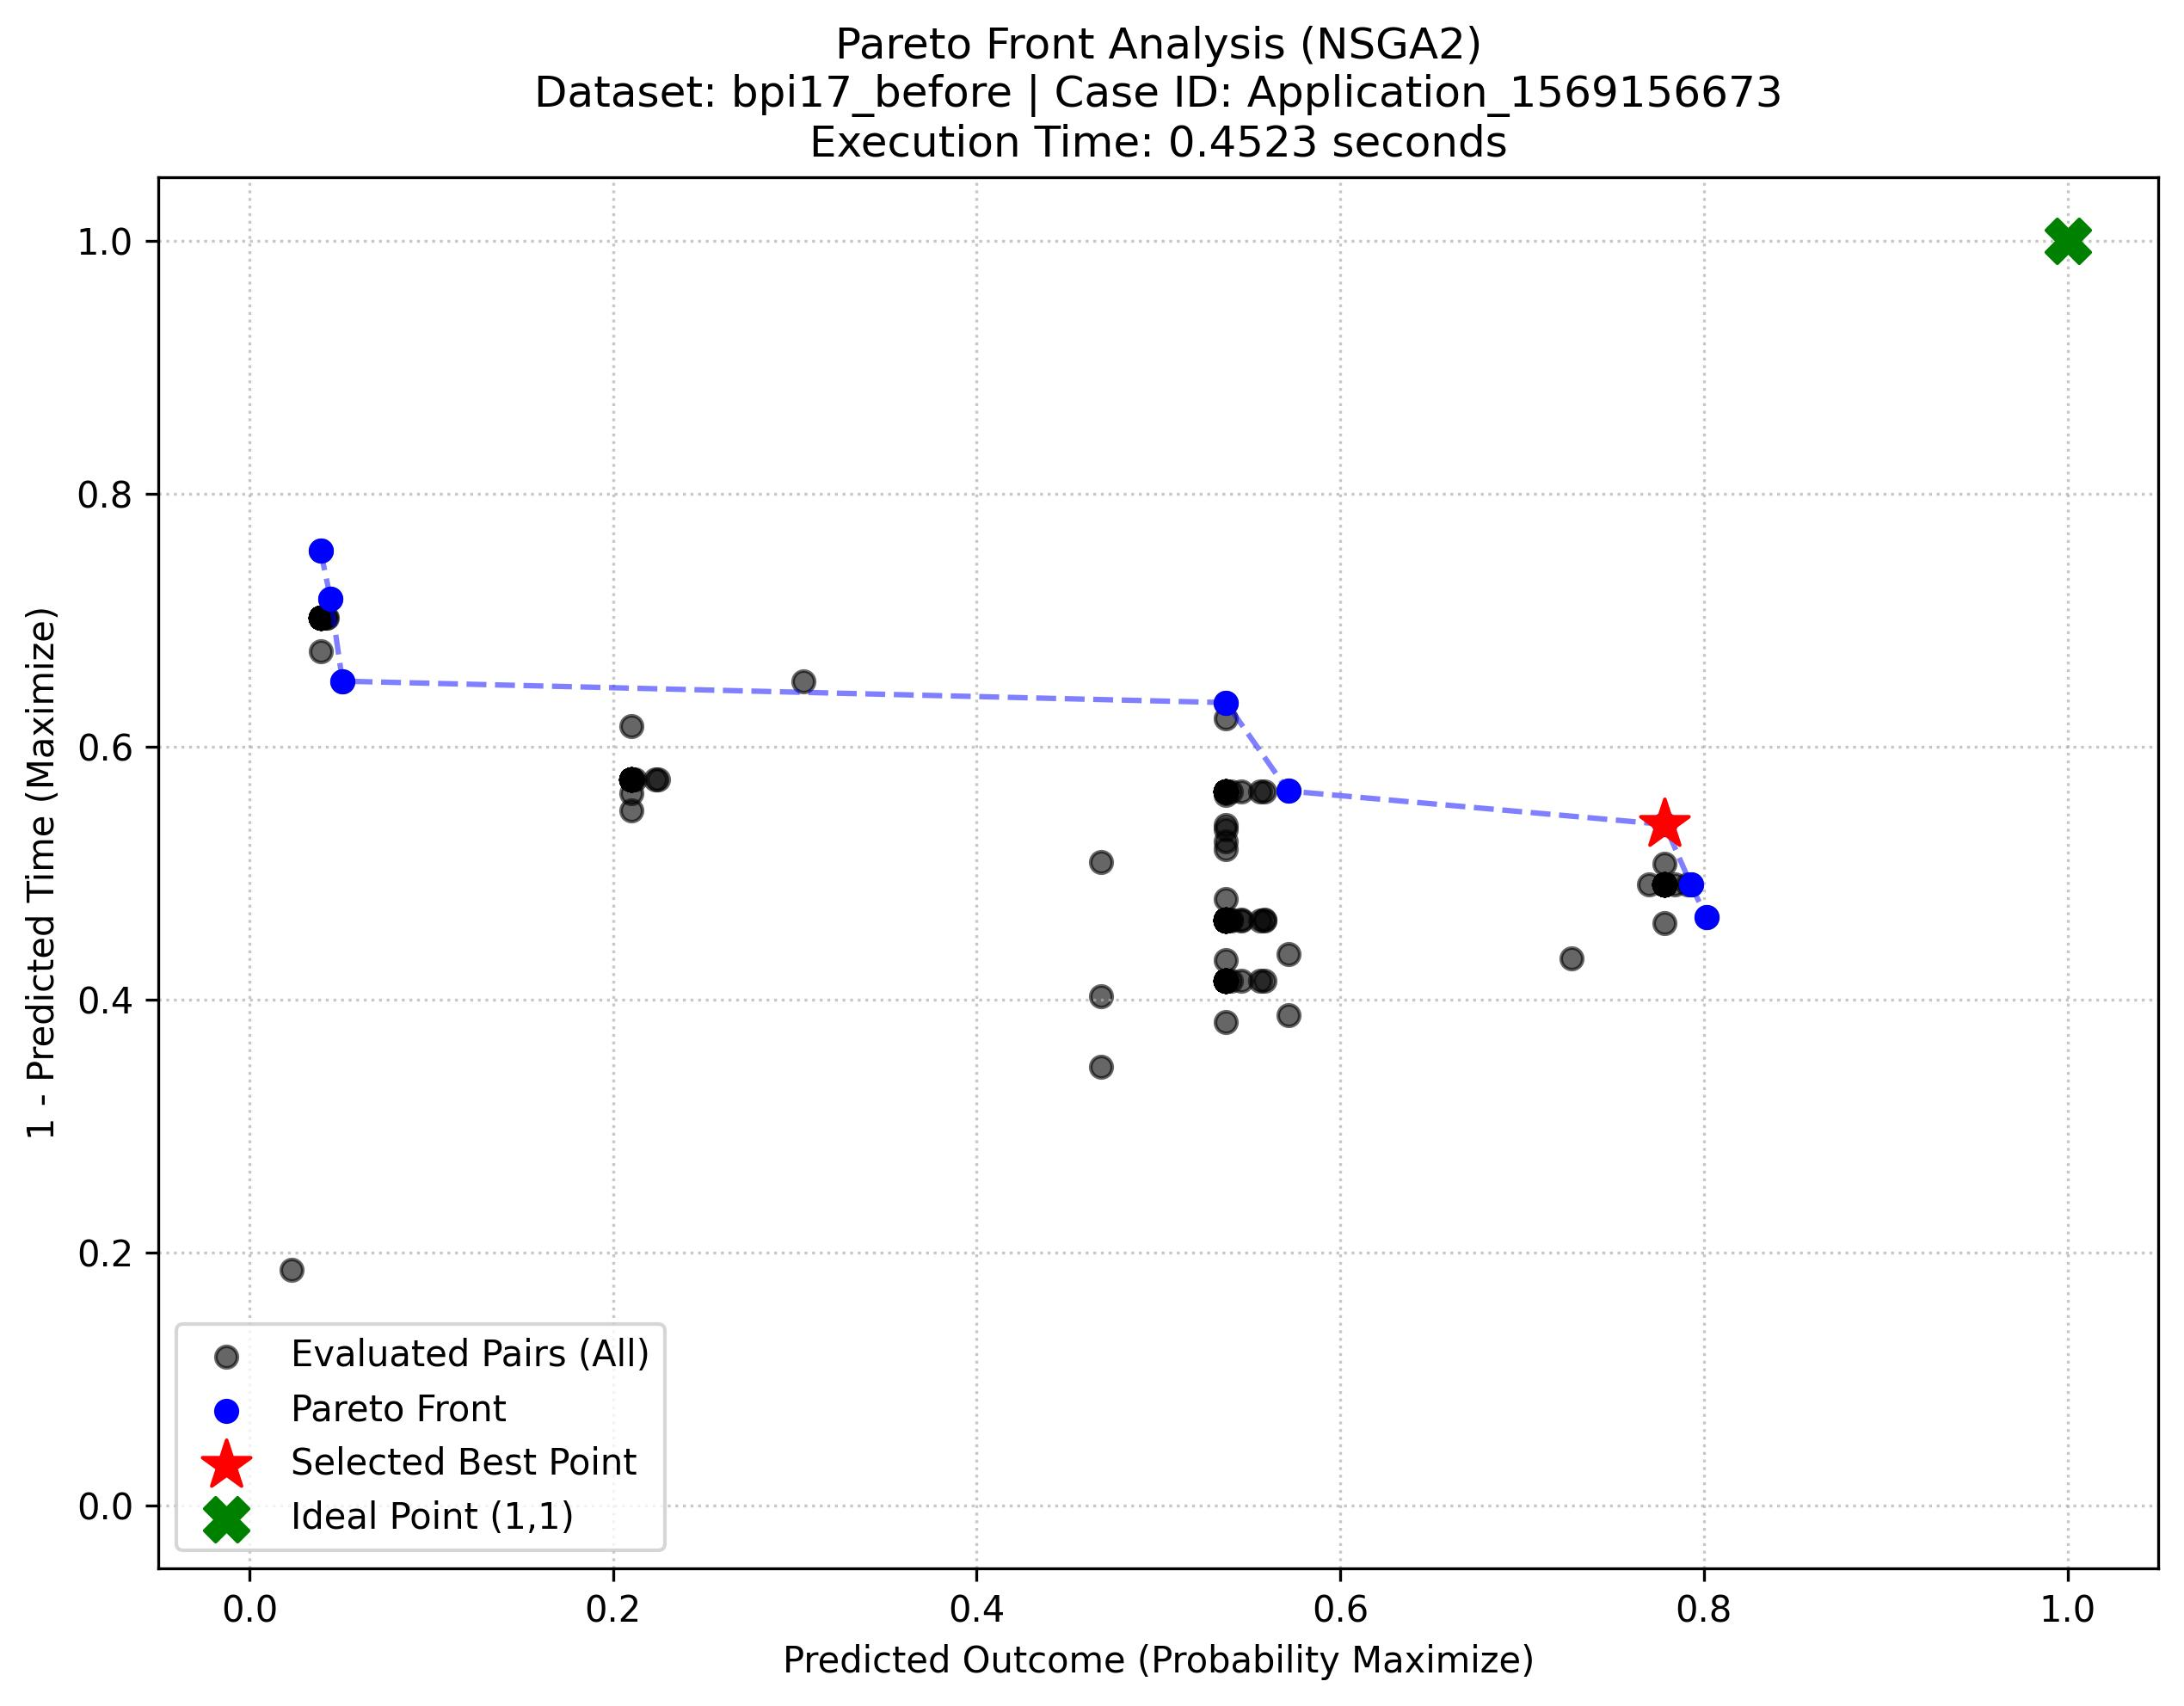
\includegraphics[width=1.03\linewidth]{pareto_front_images/pareto_bpi17_before_nsga2_Application_1569156673.jpg}
    \end{minipage}
    
\end{frame}

\begin{frame}{Experimental Results: Pareto Fronts (bpi17-after)}
    \centering
    
    \begin{minipage}{0.48\textwidth}
        \centering
        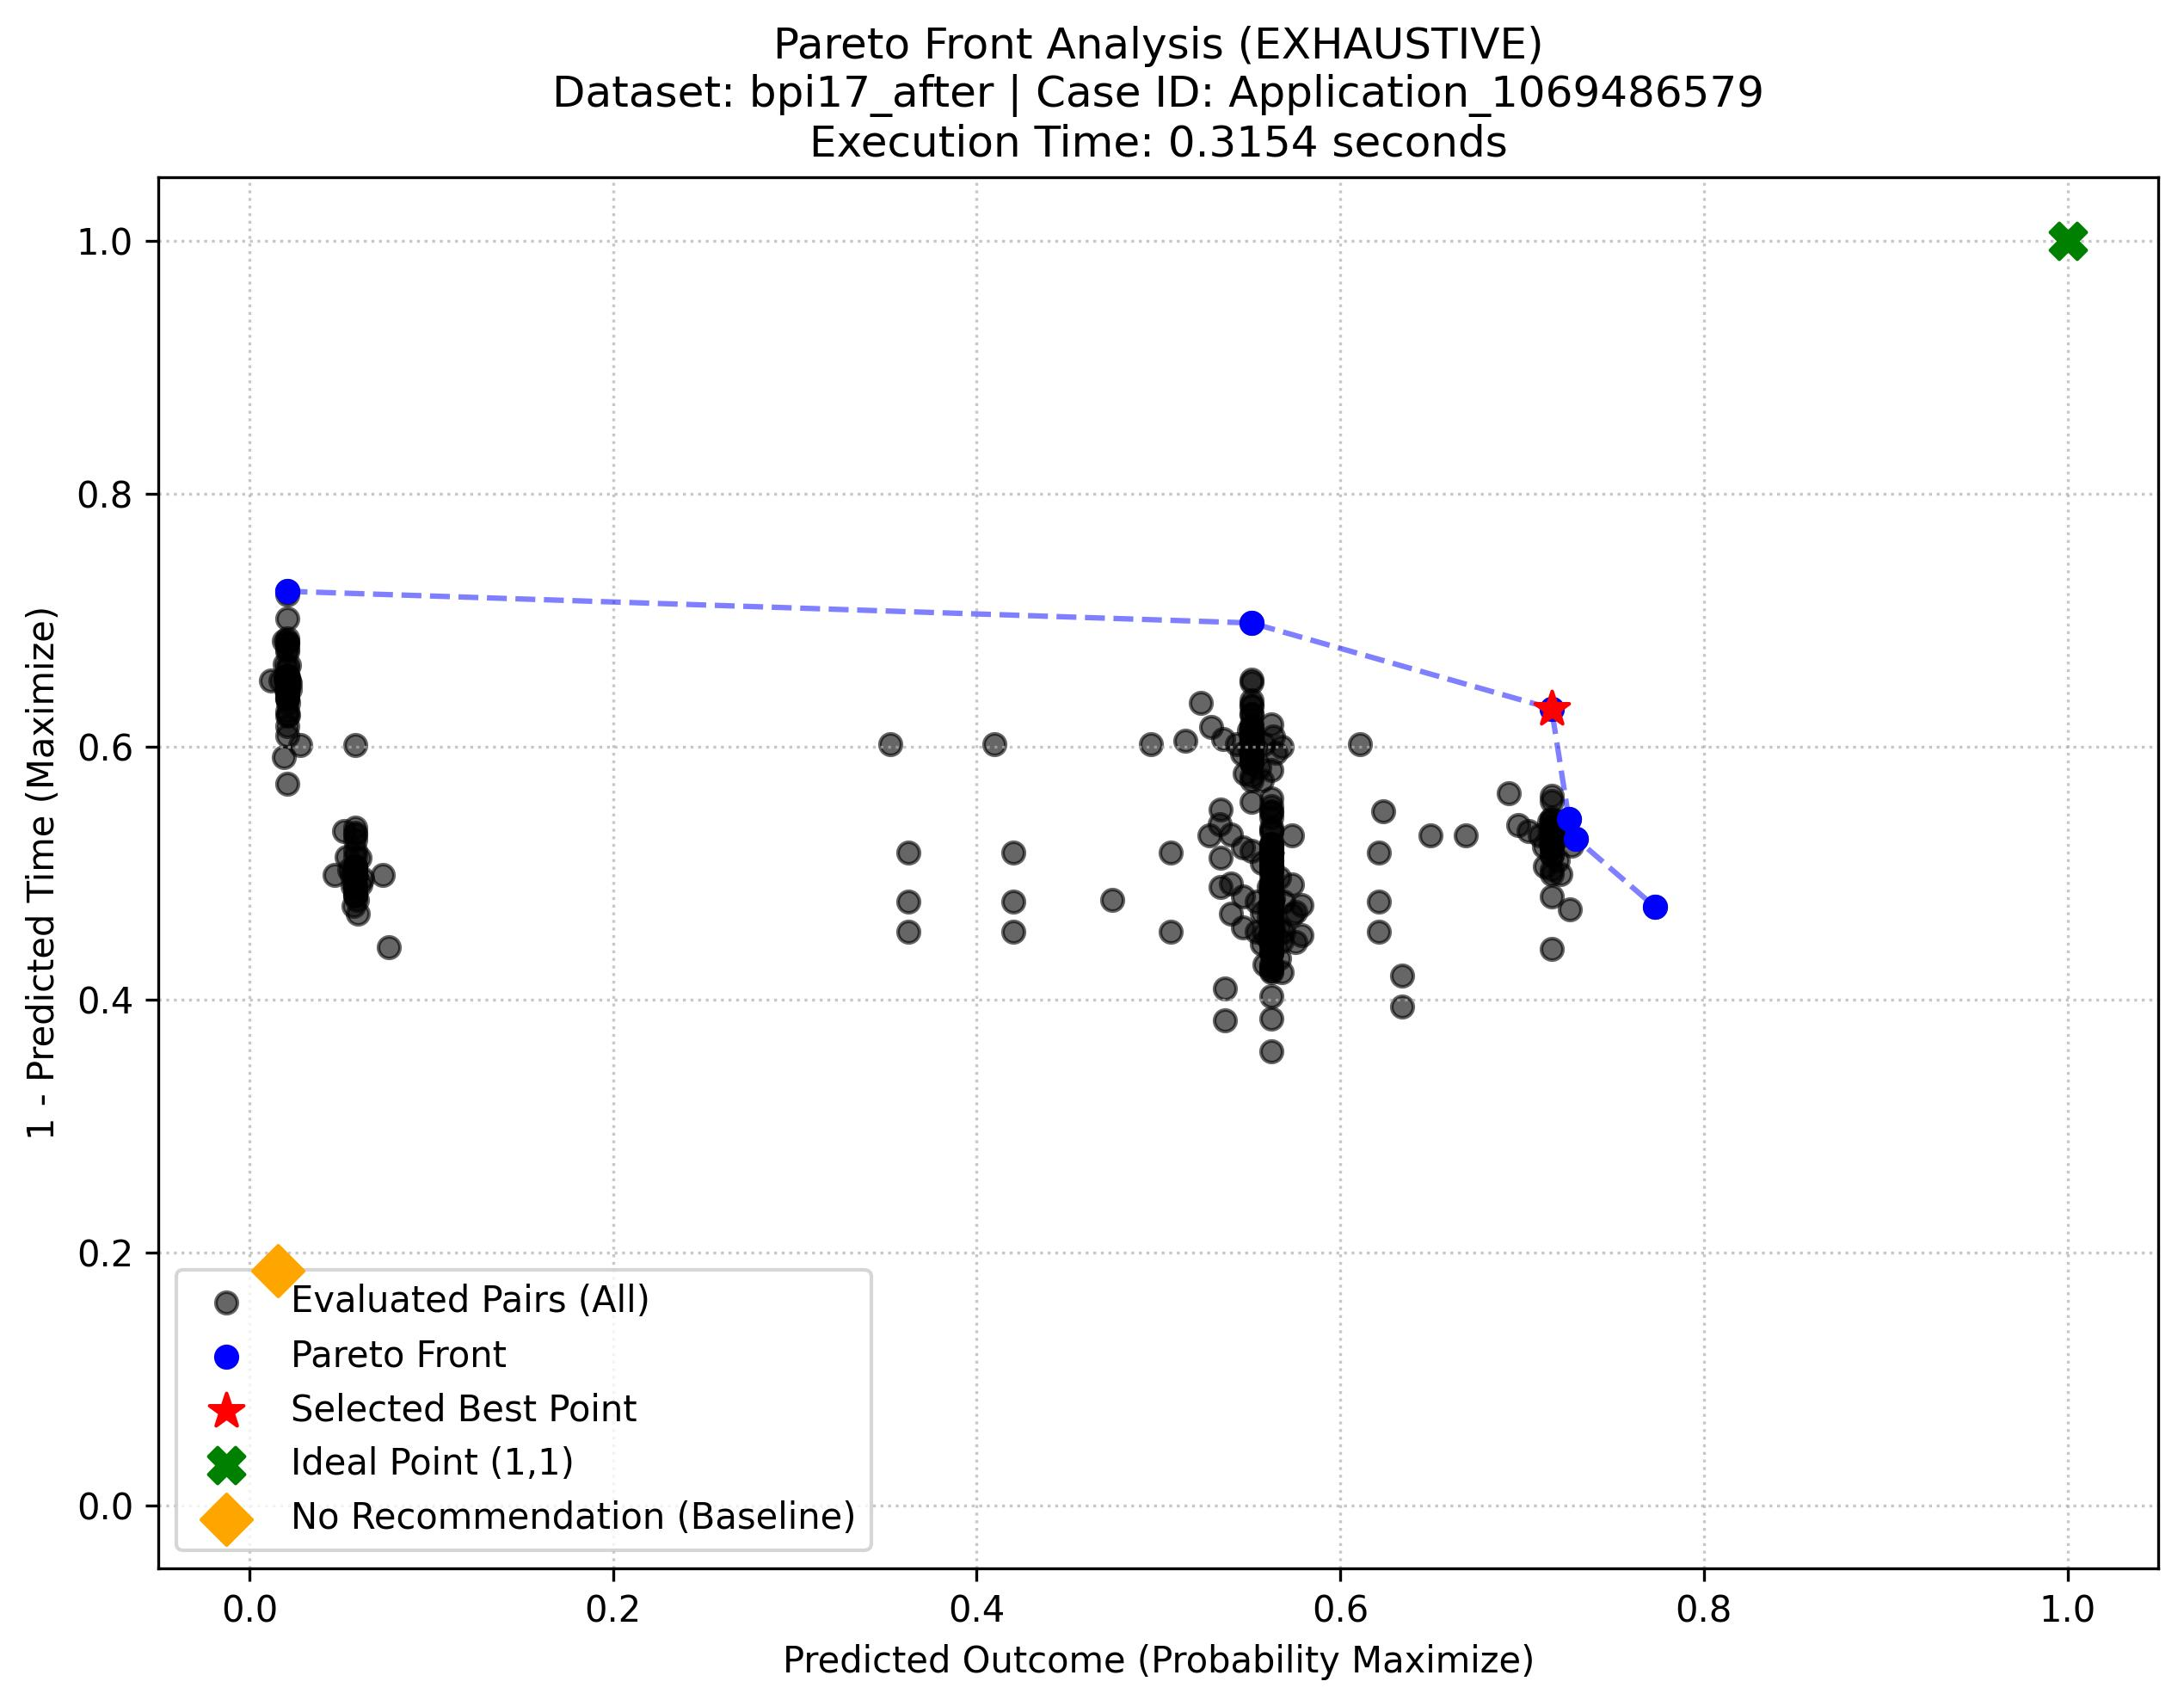
\includegraphics[width=1.03\linewidth]{pareto_front_images/pareto_bpi17_after_exhaustive_Application_1069486579.jpg}
    \end{minipage}
    \begin{minipage}{0.48\textwidth}
        \centering
        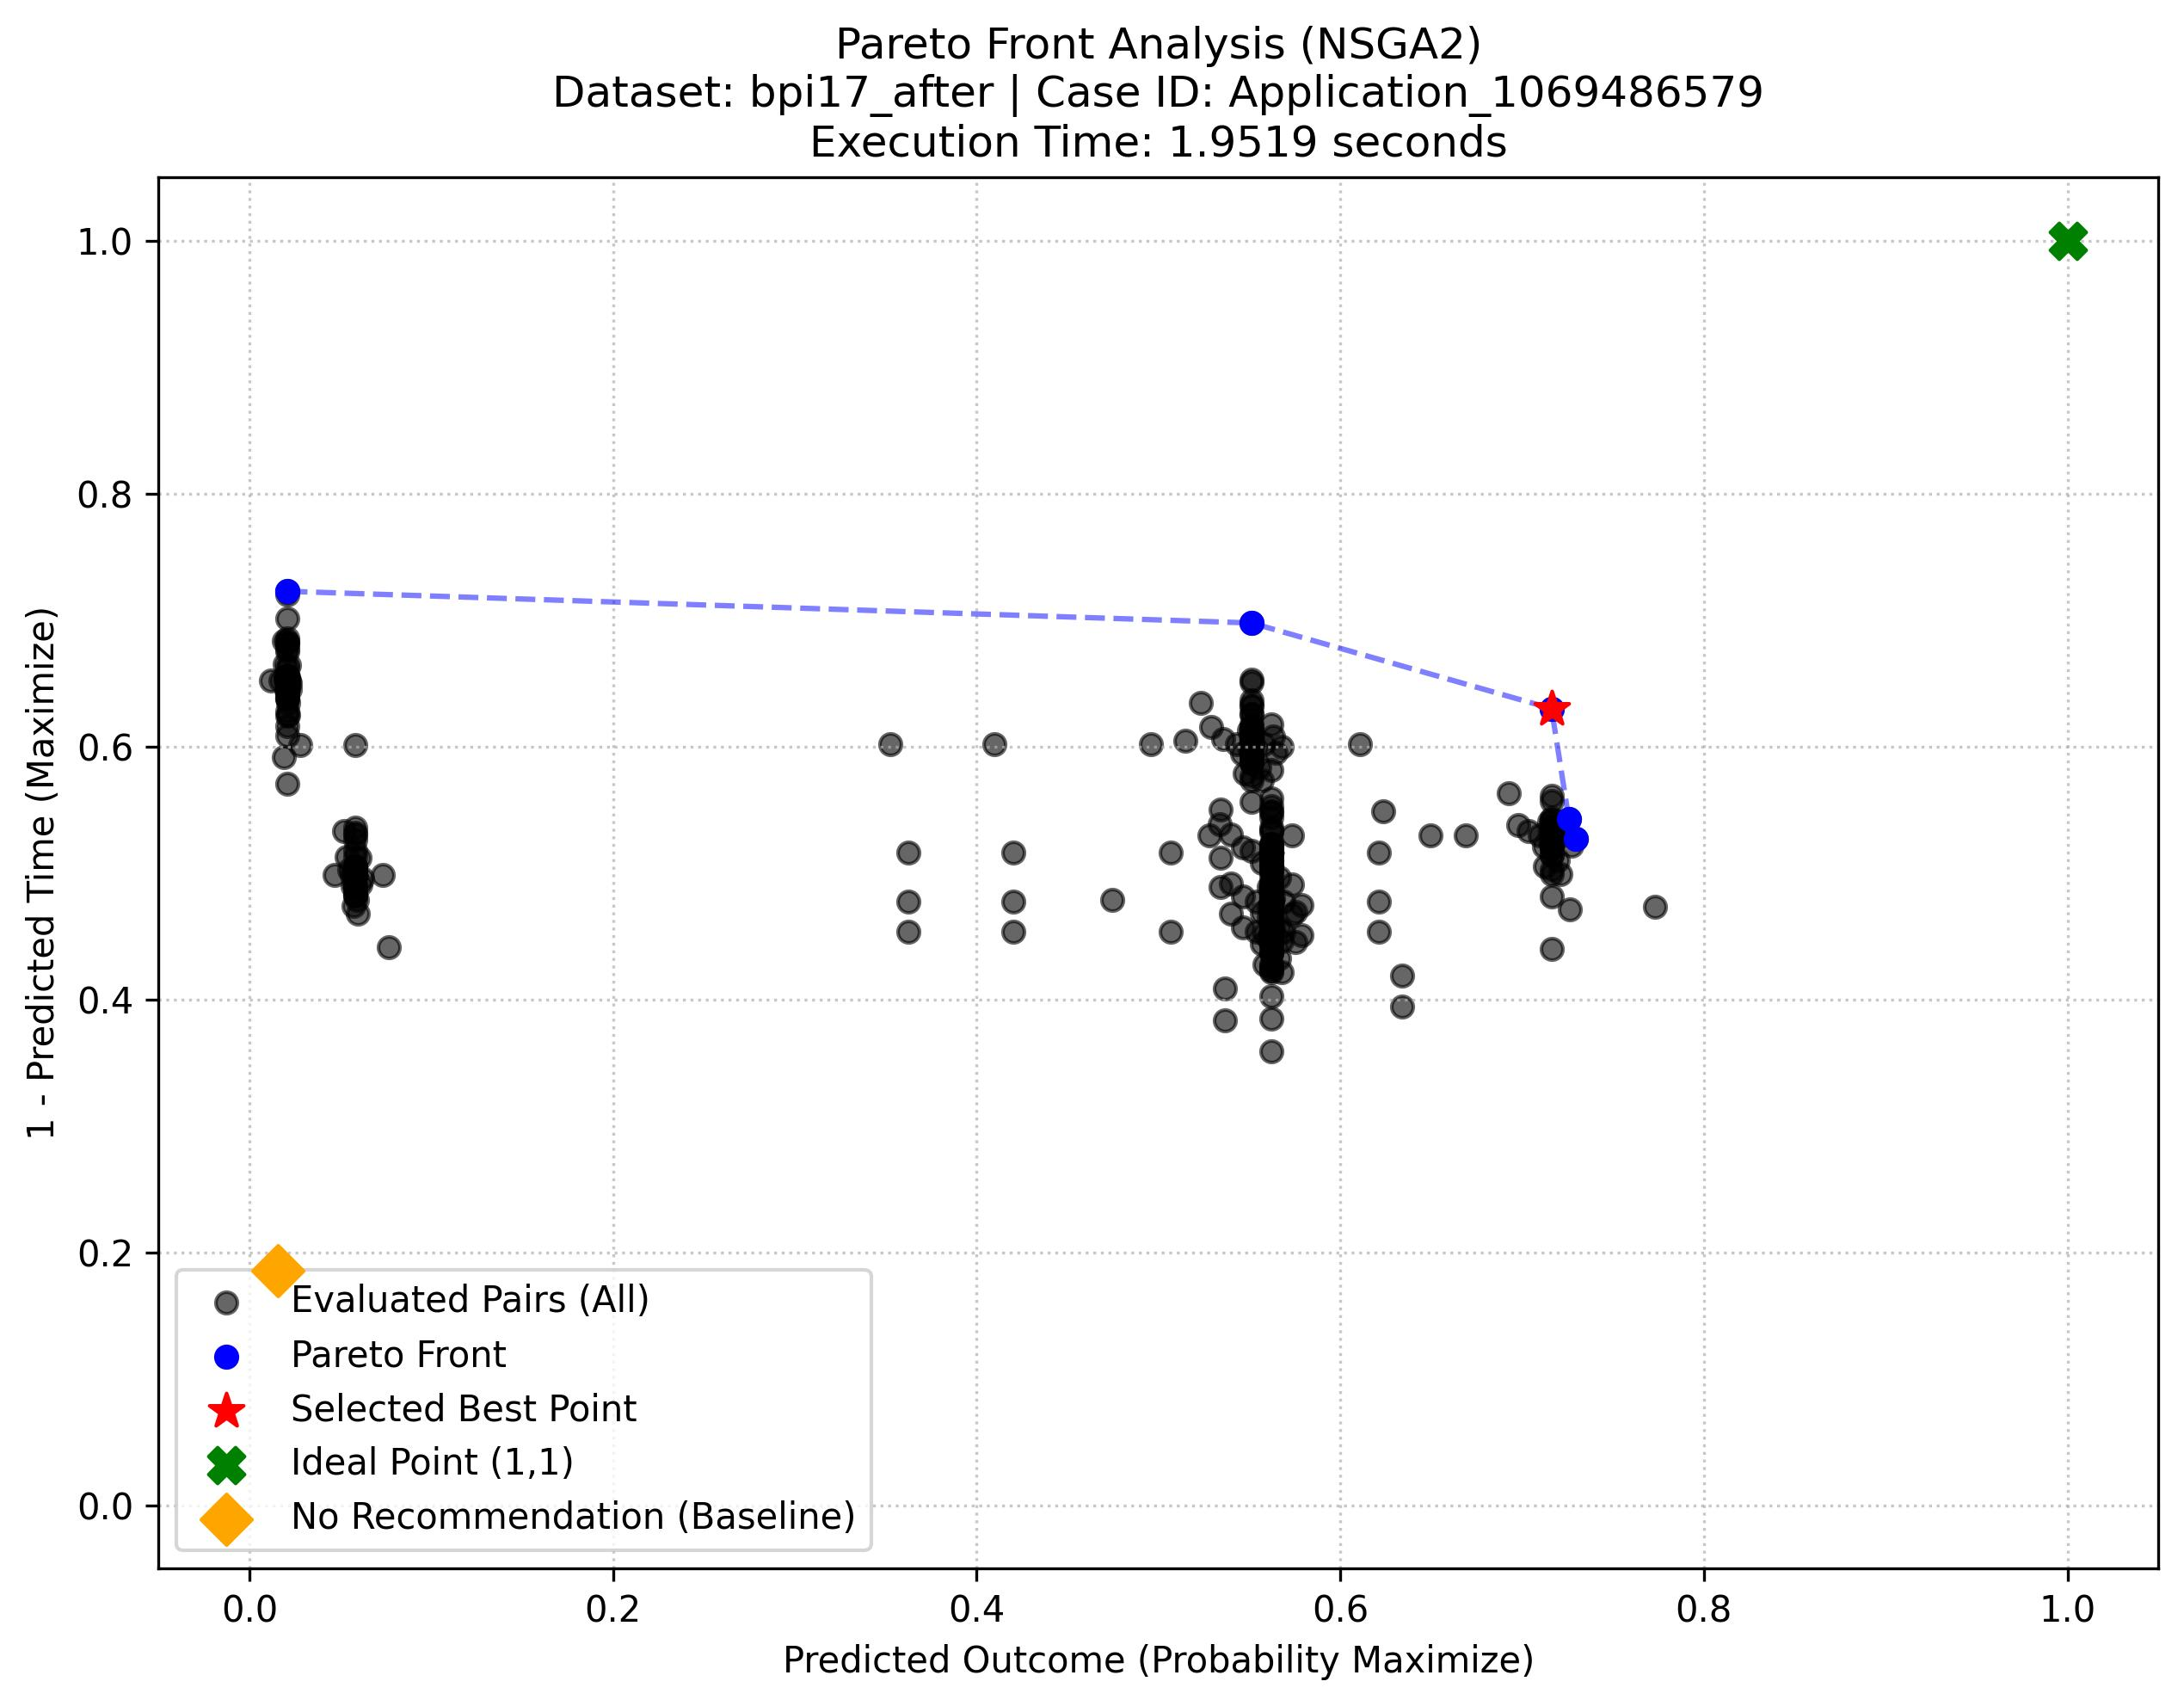
\includegraphics[width=1.03\linewidth]{pareto_front_images/pareto_bpi17_after_nsga2_Application_1069486579.jpg}
    \end{minipage}
    
\end{frame}

\begin{frame}{Simulation Pipeline (Work in Progress)}
    \begin{itemize}
        \item To evaluate the effectiveness of the \textit{a posteriori} trade-off selection, the framework is tested within a Business Process Simulation environment.
        \item \textbf{Execution Logic:}
        \begin{itemize}
            \item The framework applies the customized \textit{a posteriori} rule to pick the optimal next step from the generated Pareto front.
            \item \textbf{Simulation Loop:} The pipeline strictly iterates over individual traces sequentially to evaluate state changes, rather than re-running the entire test set.
        \end{itemize}
        \item \textit{Next Steps:} Complete simulation runs and compare the multi-model Pareto approach against the baseline.
    \end{itemize}
\end{frame}

\end{document}